% CorrTrack — three-way comparison: v1 (original) vs v1-dev (modified) vs v2 (rewrite)
% Compile: pdflatex slides_3way_v1_v1dev_v2.tex
\documentclass[aspectratio=169,10pt]{beamer}
\usepackage[T1]{fontenc}
\usepackage[utf8]{inputenc}
\usepackage{lmodern}
\usepackage{amsmath,amssymb}
\usepackage{tikz}
\usepackage{array}
\usepackage{colortbl}

\setbeamertemplate{navigation symbols}{}
\setbeamerfont{frametitle}{size=\large,series=\bfseries}

\definecolor{ink}{HTML}{14181F}
\definecolor{accent}{HTML}{2A3A57}
\definecolor{inria}{HTML}{E1000F}
\definecolor{danger}{HTML}{BD3A53}
\definecolor{ochre}{HTML}{B26A00}
\definecolor{good}{HTML}{1C8676}
\definecolor{muted}{HTML}{5C6675}
\definecolor{dangersoft}{HTML}{F8E9EC}
\definecolor{ochresoft}{HTML}{F6EEDD}
\definecolor{goodsoft}{HTML}{E6F4F1}

\setbeamercolor{frametitle}{fg=ink}
\setbeamercolor{normal text}{fg=ink}

% INRIA-red rule under each frame title (chrome only; semantic colors kept)
\setbeamertemplate{frametitle}{%
  \vspace{3pt}\usebeamerfont{frametitle}\usebeamercolor[fg]{frametitle}\insertframetitle\par
  \vspace{1pt}{\color{inria}\rule{\textwidth}{1.1pt}}\vspace{-4pt}}

\setbeamertemplate{itemize item}{\textcolor{muted}{\textbullet}}

\newcommand{\ctag}[3]{{\color{#1}\rule{1.2em}{2.2pt}}\, {\ttfamily\scriptsize\textbf{\textcolor{#1}{#2}}}\par{\tiny\textcolor{muted}{#3}}\par\vspace{2pt}}
\newcommand{\drow}[2]{\noindent\colorbox{accent}{\textcolor{white}{\tiny\,#1\,}}\ {\scriptsize #2}\par\vspace{1.2pt}}
\newcommand{\rolab}[1]{\emph{Role} --- #1\par\vspace{2pt}}
\tikzset{sc/.style={x=1mm,y=1mm,line width=.5pt,font=\tiny}}

% ---- funnel bar for the opener ----
\newcommand{\fb}[2]{\begin{tikzpicture}[baseline=0pt]\fill[#2!28](0,0)rectangle(3.1,0.16);\fill[#2](0,0)rectangle(3.1*#1,0.16);\end{tikzpicture}}
\newcommand{\fstg}[3]{{\tiny\textbf{#1}}\par\fb{#2}{#3}\par}
\newcommand{\fdn}{\vspace{-3pt}\centerline{\textcolor{muted}{\tiny$\downarrow$}}\vspace{-3pt}}

% ---- step schematics ----
\newcommand{\schemaSketch}{\centerline{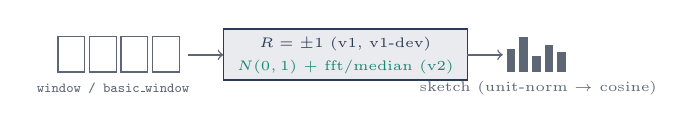
\begin{tikzpicture}[sc]
  \foreach \i in {0,1,2,3}{\draw[muted] (\i*4,0) rectangle (\i*4+3.4,4.5);}
  \node[muted,font=\tiny] at (7,-2){\ttfamily window / basic\_window};
  \draw[muted,->] (16.5,2.2)--(21,2.2);
  \draw[accent,fill=accent!10] (21,-1) rectangle (52,5.5);
  \node[accent,font=\tiny] at (36.5,3.6){$R=\pm1$ (v1, v1-dev)};
  \node[good,font=\tiny] at (36.5,0.6){$N(0,1)$ $+$ fft/median (v2)};
  \draw[muted,->] (52,2.2)--(56.5,2.2);
  \foreach \i/\h in {0/3,1/4.5,2/2,3/3.5,4/2.5}{\fill[muted] (57+\i*1.6,0) rectangle (57+\i*1.6+1.1,\h);}
  \node[muted,font=\tiny] at (61,-2){sketch (unit-norm $\to$ cosine)};
\end{tikzpicture}}}

\newcommand{\schemaIndex}{\centerline{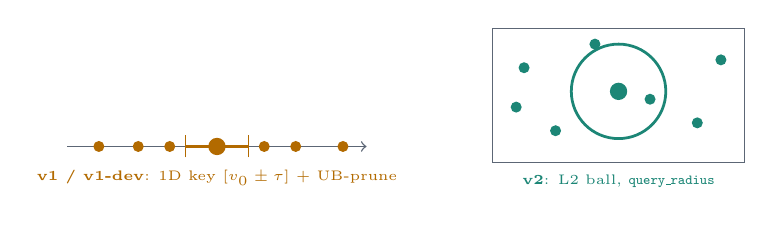
\begin{tikzpicture}[sc]
  % 1D (v1 / v1-dev)
  \draw[muted,->] (0,0)--(38,0);
  \foreach \x in {4,9,13,25,29,35}{\fill[ochre] (\x,0) circle(.7);}
  \draw[ochre,line width=1pt] (15,0)--(23,0);\draw[ochre](15,-1.4)--(15,1.4);\draw[ochre](23,-1.4)--(23,1.4);
  \fill[ochre] (19,0) circle(1.1);
  \node[ochre,font=\tiny,below] at (19,-1.8){\textbf{v1 / v1-dev}: 1D key $[v_0\pm\tau]$ $+$ UB-prune};
  % 2D (v2)
  \draw[muted] (54,-2) rectangle (86,15);
  \foreach \x/\y in {58/10,62/2,67/13,74/6,80/3,83/11,57/5}{\fill[good](\x,\y) circle(.7);}
  \fill[good] (70,7) circle(1.1);\draw[good,line width=1pt] (70,7) circle(6);
  \node[good,font=\tiny,below] at (70,-2.4){\textbf{v2}: L2 ball, \texttt{query\_radius}};
\end{tikzpicture}}}

\newcommand{\schemaAxisThree}{\centerline{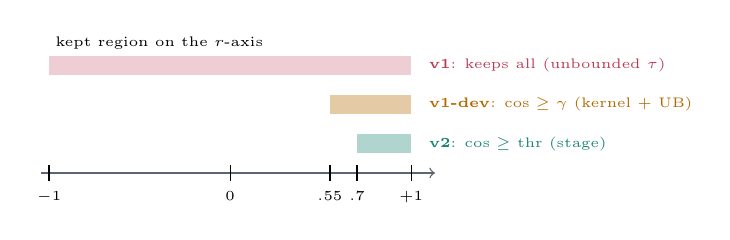
\begin{tikzpicture}[sc]
  \fill[danger!25] (0,10) rectangle (46,12.4);\node[danger,right,font=\tiny] at (47,11.2){\textbf{v1}: keeps all (unbounded $\tau$)};
  \fill[ochre!35] (35.65,5) rectangle (46,7.4);\node[ochre,right,font=\tiny] at (47,6.2){\textbf{v1-dev}: $\cos\ge\gamma$ (kernel $+$ UB)};
  \fill[good!35] (39.1,0) rectangle (46,2.4);\node[good,right,font=\tiny] at (47,1.2){\textbf{v2}: $\cos\ge$ thr (stage)};
  \draw[muted,->] (-1,-2.5)--(49,-2.5);
  \foreach \x/\l in {0/{$-1$},23/{$0$},35.65/{$.55$},39.1/{$.7$},46/{$+1$}}{\draw (\x,-3.5)--(\x,-1.5);\node[below,font=\tiny] at (\x,-3.6){\l};}
  \node[font=\tiny] at (14,14){kept region on the $r$-axis};
\end{tikzpicture}}}

\newcommand{\schemaValid}{\centerline{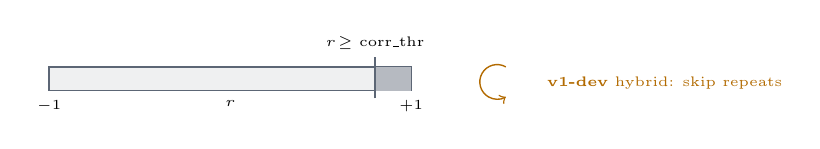
\begin{tikzpicture}[sc]
  \draw[muted,fill=muted!10] (0,0) rectangle (46,3);
  \fill[muted!45] (41.4,0) rectangle (46,3);
  \draw[muted,line width=1pt] (41.4,-1)--(41.4,4.2);\node[font=\tiny,above] at (41.4,3.9){$r\!\ge$ corr\_thr};
  \node[font=\tiny,below] at (0,0){$-1$};\node[font=\tiny,below] at (23,0){$r$};\node[font=\tiny,below] at (46,0){$+1$};
  % hybrid skip loop (v1-dev)
  \draw[ochre,->] (58,3) arc (60:300:2.2);
  \node[ochre,font=\tiny,right] at (62,1){\textbf{v1-dev} hybrid: skip repeats};
\end{tikzpicture}}}

\newcommand{\schemaTimeline}{\centerline{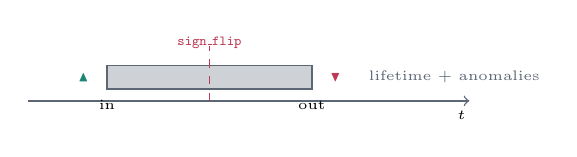
\begin{tikzpicture}[sc]
  \draw[muted,->] (0,0)--(56,0);\node[font=\tiny,below] at (55,0){$t$};
  \fill[muted!30] (10,1.5) rectangle (36,4.5);\draw[muted] (10,1.5) rectangle (36,4.5);
  \node[good,font=\tiny] at (7,3){$\blacktriangle$};\node[font=\tiny,below] at (10,1.3){in};
  \draw[danger,dashed] (23,0)--(23,7);\node[danger,font=\tiny,above] at (23,5.4){\texttt{sign\_flip}};
  \node[danger,font=\tiny] at (39,3){$\blacktriangledown$};\node[font=\tiny,below] at (36,1.3){out};
  \node[muted,font=\tiny,right] at (42,3){lifetime $+$ anomalies};
\end{tikzpicture}}}

\begin{document}
\footnotesize

% =================== OPENER: 3-way funnel ===================
\begin{frame}[t]{CorrTrack — three lineages, one pipeline}
\footnotesize
\emph{Share of pairs passing each stage (dense data). The funnel that narrows = a real filter.}
\vspace{4pt}
\begin{columns}[t]
\begin{column}{0.33\textwidth}\ctag{danger}{v1}{original --- euclidean}
\fstg{Sketch}{1.0}{danger}\fdn
\fstg{Selection (radius $\tau$)}{0.96}{danger}\fdn
\fstg{Pearson}{0.92}{danger}
\vspace{3pt}\par{\scriptsize\textcolor{danger}{$\Rightarrow$ keeps $\approx$ all $=$ brute force}}
\end{column}
\begin{column}{0.33\textwidth}\ctag{ochre}{v1-dev}{in-place --- cosine$+$UB}
\fstg{Sketch}{1.0}{ochre}\fdn
\fstg{Index (bptree)}{0.98}{ochre}\fdn
\fstg{Cosine gate $+$ UB}{0.45}{ochre}\fdn
\fstg{Pearson}{0.24}{ochre}
\vspace{3pt}\par{\scriptsize\textcolor{ochre}{$\Rightarrow$ bounded, dot-work pruned}}
\end{column}
\begin{column}{0.33\textwidth}\ctag{good}{v2}{rewrite --- modular}
\fstg{Sketch}{1.0}{good}\fdn
\fstg{Index (13 backends)}{0.98}{good}\fdn
\fstg{Cosine gate (stage)}{0.44}{good}\fdn
\fstg{Pearson}{0.23}{good}
\vspace{3pt}\par{\scriptsize\textcolor{good}{$\Rightarrow$ bounded, swappable}}
\end{column}
\end{columns}
\vspace{4pt}
\drow{thesis}{\textbf{v1} (radius, unbounded) doesn't narrow $\to$ Pearson runs on everything. \textbf{v1-dev} and \textbf{v2} bound it with a cosine gate --- by opposite routes.}
\end{frame}

% =================== OVERVIEW MATRIX ===================
\begin{frame}[t]{Overview --- v1 \; $\to$ \; v1-dev \; $\to$ \; v2}
\footnotesize
\vspace{2pt}
\renewcommand{\arraystretch}{1.32}
\setlength{\tabcolsep}{5pt}
\centerline{\begin{tabular}{@{}p{1.5cm}|p{3.5cm}|p{3.9cm}|p{3.9cm}@{}}
 & \cellcolor{dangersoft}{\ttfamily\scriptsize\textbf{\textcolor{danger}{v1}} original} & \cellcolor{ochresoft}{\ttfamily\scriptsize\textbf{\textcolor{ochre}{v1-dev}} in-place} & \cellcolor{goodsoft}{\ttfamily\scriptsize\textbf{\textcolor{good}{v2}} rewrite}\\[1pt]
\hline
{\scriptsize\textbf{Sketch}} & {\scriptsize Rademacher $\pm1$ RP $+$ toggle} & {\scriptsize same RP, unit-norm for cosine} & {\scriptsize Gaussian $+$ \textbf{5 methods}, swappable}\\
{\scriptsize\textbf{Index}} & {\scriptsize \texttt{bptree}/\texttt{flat}, 1D key} & {\scriptsize \texttt{bptree} $+$ UB-prune infra} & {\scriptsize \textbf{13 indexes}, cdist batch}\\
{\scriptsize\textbf{Selection}} & {\scriptsize \textbf{euclidean radius} (unbounded)} & {\scriptsize \textbf{cosine} $\gamma$ fused $+$ UB, $|\cos|$} & {\scriptsize \textbf{cosine} gate stage, cdist, $|\cos|$}\\
{\scriptsize\textbf{Validation}} & {\scriptsize Pearson $+$ kurtosis $+$ min\_dist} & {\scriptsize $+$ \textbf{hybrid} adaptive skip} & {\scriptsize \texttt{correlate}, std only, signed lag}\\
{\scriptsize\textbf{Monitoring}} & {\scriptsize in/out, Cython kernel} & {\scriptsize $+$ numeric fast path} & {\scriptsize \texttt{Monitor}, pure bookkeeping}\\
\end{tabular}}
\vspace{5pt}
\drow{v1 $\to$ v1-dev}{in-place: euclidean $\to$ \textbf{cosine gate} fused in the Cython kernel $+$ Cauchy--Schwarz UB pruning, single-insert.}
\drow{v1 $\to$ v2}{modular rewrite: separate cosine stage, 13 swappable indexes, backend-swappable compute, 5 sketch methods.}
\drow{v1-dev $\approx$ v2}{same selection idea (cosine, single-insert) --- v1-dev \textbf{deep-optimizes the monolith}, v2 \textbf{modularizes}.}
\end{frame}

% =================== 1. SKETCH ===================
\begin{frame}[t]{Step 1 — Sketch: projecting the window}
\footnotesize
\rolab{turn each window into a short vector ($n\_vectors$) that preserves correlation (JL projection).}
\schemaSketch
\vspace{5pt}
\begin{columns}[t]
\begin{column}{0.32\textwidth}\ctag{danger}{v1}{original}
{\scriptsize\begin{itemize}\setlength\itemsep{1pt}
\item \textbf{Rademacher} $\pm1$ $+$ toggle
\item norm \texttt{z} $|$ \texttt{mean\_l2}, Cython
\end{itemize}}
\end{column}
\begin{column}{0.32\textwidth}\ctag{ochre}{v1-dev}{in-place}
{\scriptsize\begin{itemize}\setlength\itemsep{1pt}
\item \textbf{same} RP $+$ toggle
\item \textbf{unit-norm} $\to$ dot $=$ cosine
\end{itemize}}
\end{column}
\begin{column}{0.32\textwidth}\ctag{good}{v2}{rewrite}
{\scriptsize\begin{itemize}\setlength\itemsep{1pt}
\item Gaussian $N(0,1)$ $+$ \texttt{znormalize}
\item \textbf{5 methods}: RP, fft, median
\end{itemize}}
\end{column}
\end{columns}
\vspace{4pt}
\drow{v1 $\to$ v1-dev}{same projection; normalization becomes unit ($\ell_2$) so the candidate dot equals the cosine.}
\drow{v1-dev $\to$ v2}{same RP idea; v2 adds sketch \emph{variety} (FFT/median $=$ AUC lever) $+$ swappable backend.}
\end{frame}

% =================== 2. INDEX ===================
\begin{frame}[t]{Step 2 — Index / neighbor retrieval}
\footnotesize
\rolab{for each window, find its neighbors in sketch space (raw candidates).}
\schemaIndex
\vspace{4pt}
\begin{columns}[t]
\begin{column}{0.32\textwidth}\ctag{danger}{v1}{original}
{\scriptsize\begin{itemize}\setlength\itemsep{1pt}
\item \texttt{bptree}/\texttt{flat}, 1D key
\item range $+$ L2 refine
\end{itemize}}
\end{column}
\begin{column}{0.32\textwidth}\ctag{ochre}{v1-dev}{in-place}
{\scriptsize\begin{itemize}\setlength\itemsep{1pt}
\item \texttt{bptree} (AVL), 1D key
\item $+$ \textbf{UB-prune} (skip dots)
\end{itemize}}
\end{column}
\begin{column}{0.32\textwidth}\ctag{good}{v2}{rewrite}
{\scriptsize\begin{itemize}\setlength\itemsep{1pt}
\item \textbf{13 indexes} (grid/bst/hnsw…)
\item BLAS cdist batch
\end{itemize}}
\end{column}
\end{columns}
\vspace{4pt}
\drow{v1 $\to$ v1-dev}{same \texttt{bptree}; the scan gains a Cauchy--Schwarz \textbf{upper bound} to skip full dot products.}
\drow{v1-dev $\to$ v2}{v1-dev \textbf{prunes work} in one smart tree; v2 \textbf{swaps} among many brute-but-vectorized indexes.}
\end{frame}

% =================== 3. SELECTION / GATE ===================
\begin{frame}[t]{Step 3 — Selection / cosine gate: what each keeps}
\footnotesize
\vspace{-1pt}
\schemaAxisThree
\vspace{1pt}
\begin{columns}[t]
\begin{column}{0.32\textwidth}\ctag{danger}{v1}{original}
{\scriptsize\begin{itemize}\setlength\itemsep{0pt}
\item \textbf{euclidean} \texttt{cell\_size} $(\tau)$
\item $r\gtrsim1-\tau^2/2$, \textbf{unbounded}
\item double-insert $-vec$
\end{itemize}}
\end{column}
\begin{column}{0.32\textwidth}\ctag{ochre}{v1-dev}{in-place}
{\scriptsize\begin{itemize}\setlength\itemsep{0pt}
\item \textbf{cosine} $\gamma$ \textbf{fused in kernel}
\item $\gamma=1-\tau^2/2$ (overridable) $+$ UB
\item single-insert $|\cos|$
\end{itemize}}
\end{column}
\begin{column}{0.32\textwidth}\ctag{good}{v2}{rewrite}
{\scriptsize\begin{itemize}\setlength\itemsep{0pt}
\item \textbf{cosine} gate \emph{separate} stage
\item \texttt{sketch\_threshold}, cdist
\item single-insert $|\cos|$
\end{itemize}}
\end{column}
\end{columns}
\vspace{2pt}
\drow{v1 $\to$ v1-dev/v2}{unbounded radius $\to$ \textbf{bounded cosine} $\to$ v1's ``keep everything'' becomes inexpressible.}
\drow{shared limit}{$\cos\approx r$ is noisy: recall $0.95 \Rightarrow \gamma\approx0.55$ (not $0.7$) $\Rightarrow$ wide band $[0.55,0.7)$ for both.}
\end{frame}

% =================== 4. VALIDATION ===================
\begin{frame}[t]{Step 4 — Exact Pearson validation}
\footnotesize
\rolab{exact correlation on raw windows: confirm or reject each candidate.}
\schemaValid
\vspace{4pt}
\begin{columns}[t]
\begin{column}{0.32\textwidth}\ctag{danger}{v1}{original}
{\scriptsize\begin{itemize}\setlength\itemsep{1pt}
\item \texttt{fast\_corr\_and\_dist}
\item std$<10^{-3}$, kurt$>5$, min\_dist
\end{itemize}}
\end{column}
\begin{column}{0.32\textwidth}\ctag{ochre}{v1-dev}{in-place}
{\scriptsize\begin{itemize}\setlength\itemsep{1pt}
\item \textbf{same} Pearson $+$ guards
\item $+$ \textbf{hybrid} skip (EMA repeat)
\end{itemize}}
\end{column}
\begin{column}{0.32\textwidth}\ctag{good}{v2}{rewrite}
{\scriptsize\begin{itemize}\setlength\itemsep{1pt}
\item \texttt{backend.correlate} (swappable)
\item \texttt{std\_threshold}, signed lag
\end{itemize}}
\end{column}
\end{columns}
\vspace{4pt}
\drow{v1 $\to$ v1-dev}{same exact Pearson; a \textbf{hybrid} layer skips re-validating stable, repeating pairs.}
\drow{v1-dev $\to$ v2}{v1-dev cuts validation \emph{count} (hybrid); v2 cuts \emph{cost/pair} (vectorized swappable backend).}
\end{frame}

% =================== 5. MONITORING ===================
\begin{frame}[t]{Step 5 — Persistence monitoring}
\footnotesize
\rolab{track over time the lifetime of correlations and their anomalies (onset, drop, sign change).}
\schemaTimeline
\vspace{4pt}
\begin{columns}[t]
\begin{column}{0.32\textwidth}\ctag{danger}{v1}{original}
{\scriptsize\begin{itemize}\setlength\itemsep{1pt}
\item \texttt{corr\_lengths}/\texttt{anomalies}
\item \texttt{\_in\_corr}/\texttt{\_out\_corr}, Cython
\end{itemize}}
\end{column}
\begin{column}{0.32\textwidth}\ctag{ochre}{v1-dev}{in-place}
{\scriptsize\begin{itemize}\setlength\itemsep{1pt}
\item \textbf{same} model (in/out)
\item $+$ \textbf{numeric fast path}
\end{itemize}}
\end{column}
\begin{column}{0.32\textwidth}\ctag{good}{v2}{rewrite}
{\scriptsize\begin{itemize}\setlength\itemsep{1pt}
\item \texttt{Monitor} class, typed anomalies
\item \textbf{pure bookkeeping}, no backend
\end{itemize}}
\end{column}
\end{columns}
\vspace{4pt}
\drow{v1 $\to$ v1-dev}{same lifetime model; a numeric fast path added to the existing Cython monitoring.}
\drow{v1-dev $\to$ v2}{v1-dev keeps the coupled Cython$+$spill design; v2 \textbf{decouples} it into pure state.}
\end{frame}

\end{document}
